\subsubsection{Python als Progrmmiersprache}

Nach dem Scheitern seiner ersten Programmiersprache entwickelte Guido van Rossum die Sprache Python, dabei wollte er alle Fehler, die er beim Entwickeln von ABC gefunden hat, verbessern. Daher basieren auch die Strukturen und Konventionen von Python auf Unix, ohne an Unix gebunden zu sein. \cite{PythonGVR:online}

Python unterscheidet sich in vielen Punkten zu anderen Sprachen, unter anderem, dass sie viel Wert auf Lesbarkeit legt. Die auffälligste davon ist, dass Einrückungen Codeblöcke unterteilen anstatt eine Art von Klammern. Dafür gibt es zwei Gründe:

\begin{itemize}
    \item Es macht den Code kürzer und er wirkt nicht unnötig ausgeschmückt, daher braucht man eine kürzere Aufmerksamkeitsspanne, um den Sinn einer Codestelle nachvollziehen zu können.
    \item Die Struktur des Codes ist vereinheitlicht, was es einfacher macht, Projekte von anderen zu verstehen.
\end{itemize}

Außerdem werden dem Entwickler in vielen Entscheidungen leichter gemacht, da unnötige Möglichkeiten entfernt wurden, das heißt, dass es meistens nur eine offensichtliche Art und Weise gibt, etwas zu implementieren. Dazu kommt noch die Nutzung von Spezialzeichen. Es werden nur Zeichen unterstützt, die den meisten bereits bekannt sind und dessen Operation Sinn machen. \cite{PythonGVR:online}

Dies beantwortet jedoch nicht die Frage ''Wieso ist Python die beliebteste Sprache für \gls{ml}?''. Die Antwort darauf ist, dass nicht nur triviale Aufgaben bereits vorimplementiert, sondern auch, dass die meisten ML Funktionen in Python Libraries zusammengefasst sind. Daher muss man als Neuanfänger oder Fortgeschrittener keine bereits gelösten Probleme von Grund auf noch einmal angehen.

\subsubsection{Notebooks}

Da es bei \gls{ml} öfters dazu kommt, dass bestimmte Codeblöcke oft wiederholt ausgeführt werden, kann man mithilfe von Notebooks diese einzeln ausführen. Zum Beispiel beim Analysieren eines Datensatzes oder um schnell kleine Änderung am geplanten Vorgehen vorzunehmen.

Diese Codeblöcke können entweder Code, Texte oder Grafiken beinhalten, diese werden fortlaufend mit einer Nummer versehen und die Ausgabe/Grafik erscheint direkt unter dem Code.

\begin{figure}[H]
    \centering
    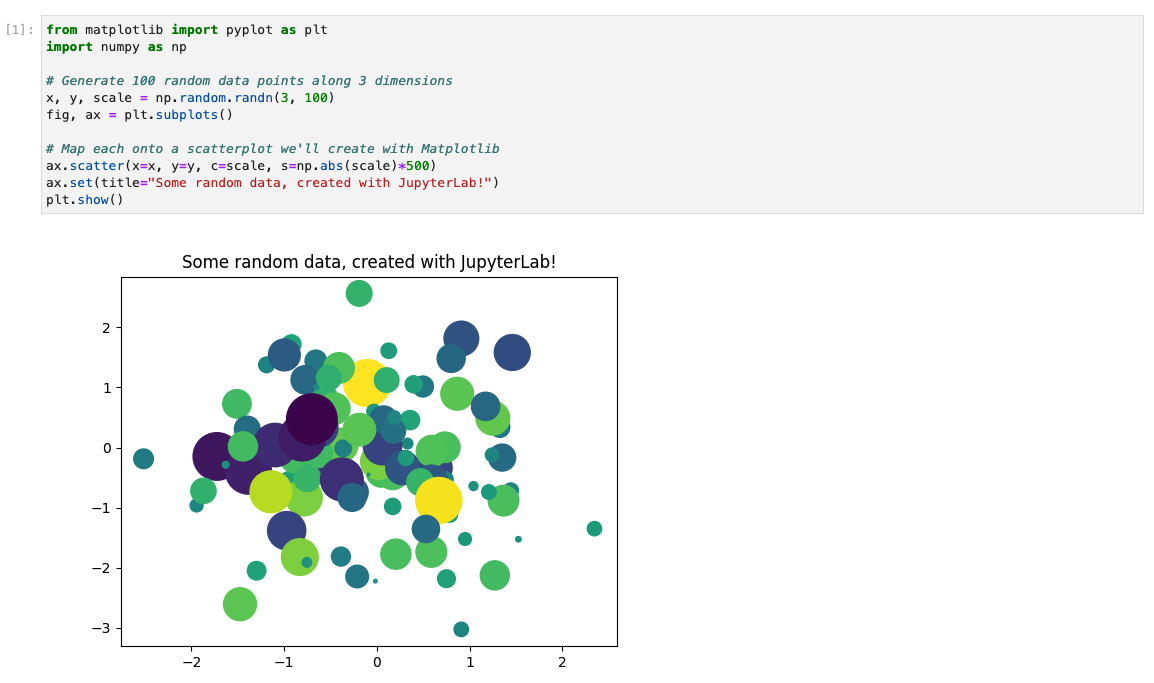
\includegraphics[scale=0.4]{sections/machine-learning/images/jupyter-notebook.png}
    \caption{Beispiel für ein Notebook mit Code und Ausgabe mit Jupyter Notebook}
\end{figure}

Diese Notebooks kann man entweder lokal starten oder auf diversen Webseiten online benutzen, dann wird auch der Code auf den Servern dieser Notebookseiten ausgeführt. Dies kann von großem Vorteil sein, da oft generierte Grafiken sehr viel Leistung in Anspruch nehmen. Außerdem werden die Ergebnisse/Ausgaben gespeichert und man muss nicht bei jedem Neuladen jeden Codeblock neu ausführen.

\subsubsection{Libraries}

\paragraph{Pandas}

Bevor der eigentliche ML-Prozess beginnen kann, müssen die Daten als Erstes analysiert werden und dafür ist die Library ''pandas'' geeignet. Neben der Analyse ist pandas auch in der Datenmanipulation sehr hilfreich, da die vordefinierten Funktionen nicht nur leicht und verständlich, sondern auch für echte Daten aus der Welt gedacht, sind.

Zu den zwei Hauptdatentypen von pandas gehören Dataframes und Series.

\subparagraph{Series} sind eindimensionale Arrays, welche aus verschiedenen Datentypen bestehen können. Mithilfe von einer ID kann man auf jeden Eintrag in der Series zugreifen, diese sind entweder mitgegeben worden oder von pandas generiert (aufsteigende Zahl beginnend bei 0).

Mit der Methode \lstinline!pandas.Series(data)! können Dictionaries, ndarrys und Skalarwerte in Series umgewandelt werden.

\subparagraph{Dataframes} sind zweidimensionale Tabellen mit verschiedenen Datentypen als Spalten. Sie sind vergleichbar mit Datenbanktabellen oder mit einem Dictionary mit dem Datentyp Series als Value.

Jede Zeile beinhaltet eine ID, falls diese nicht vergeben ist, wird von pandas eine generiert und mittels dieser ID kann man dann auf bestimmte Zeilen zugreifen. Das gleiche Prinzip gilt bei den Spalten, wo man mit der Spaltenbezeichnung auf jeden Wert der Zeilen assoziiert und mit dieser Spalte zugreifen kann.

pandas bietet beim Erstellen von Dataframes mehrere Möglichkeiten an: \cite{pandas}

\begin{itemize}
    \item Einlesen einer Datei (*.json, *.html, *.sql, *.xlsx, ...)

          Am Beispiel einer .csv-Datei: \lstinline!pandas.read_csv(FILENAME)!
    \item Dictionaries

          \lstinline!pandas.DataFrame.from_dict(DICT_VARIABLE)!
    \item Series

          \lstinline!pandas.Series.to_frame(SERIES_VARIABLE)!
    \item Anderes Dataframe
\end{itemize}

Das Benutzen von pandas erspart sehr viel Zeit und ermöglicht den schnellsten Weg zu einem Ergebnisse mit diesen Funktionalitäten:

\begin{itemize}
    \item Löschen und Ersetzen von fehlenden Daten, was beim Vorbereiten der Daten hilfreich ist 
    \item Hinzufügen und Löschen von Spalten in Dataframes
    \item Gruppierung von Daten
    \item Koventierung in NumPy oder andere Python Objekte
    \item ...
\end{itemize}

\paragraph{spaCy}

spaCy ist eine Library, die beim Implementieren von \gls{nlp}-Modell vieles vereinfacht. Mit der Veröffentlichung in 2015 überholte es schnell die zu der Zeit meistgenutzte \gls{nlp}-Library NLTK. Als öffentliche Library wurde sie immer vermehrt in privaten als auch kommerziellen Projekten verwendet. \cite{NER-NLP}

Mit dem Download von spaCy werden insgesamt 64 Sprachen mitgeliefert, welche bereits mit einem \gls{nlp}-Modell referenziert sind. Diese Modelle wurden mit einer großen Menge an Daten für unterschiedliche Bereiche trainiert. Reichen diese jedoch nicht, gibt es immer die Möglichkeit, ein bereits Existierendes anzupassen oder ein komplett Neues zu erstellen. \cite{NER-NLP}

spaCy stellt sogar ein antrainiertes \gls{ner}-Modell zur Verfügung, welches Entitäten erkennt, die im kommerziellen Bereich oft zum Beispiel in Verträgen, Artikeln oder Rechnungen vorkommen. Die in Tabelle \ref{spacy:entities} aufgezählten Entitäten, werden mithilfe von einem vortrainierten \gls{ner}-Modell erkannt.

Das Endergebnis kann aus mehreren Zeilen bestehen und setzt sich aus vier Teilen zusammen. Zuerst der eigentliche Text, danach der Startindex und Endindex im Text und zum Schluss die erkannte Entität.

\begin{lstlisting}[caption={Beispiel für ein spaCy NER Ergebnis}]
    [
        ('fb', 0, 1, 'ORG'),
        ('Barack Obama', 13, 25, 'PERSON'),
        ('Wels', 94, 98, 'GPE'),
        ('1994', 0, 4, 'DATE')
    ]
\end{lstlisting}

Zu diesen zuvor antrainierten Entitäten gehören: \cite{NER-NLP}

\begin{table}[H]
    \centering
    \begin{tabular}{|l|l|}
    \hline
    PERSON      & Person (Name)                                        \\ \hline
    NORP        & Nationalitäten oder religiöse oder politische Gruppe \\ \hline
    FAC         & Gebäude, Flughafen, Brücken, ...                     \\ \hline
    ORG         & Unternehmen, Agentur, Institution, ...               \\ \hline
    GPE         & Länder, Städte, Bundesstaaten                        \\ \hline
    LOC         & Nicht GPE Orte (Meere, Seen, Berggruppen)            \\ \hline
    PRODUCT     & Objekte, Fahrzeuge, Essen, ...                       \\ \hline
    EVENT       & Kriege, Kämpfe, Sport Events, ...                    \\ \hline
    WORK\_OF\_ART & Büchertitel, Songs                                 \\ \hline
    LAW         & Gesetze                                              \\ \hline
    LANGUAGE    & Sprachen                                             \\ \hline
    DATE        & Datum                                                \\ \hline
    TIME        & Uhrzeiten, die kleiner als ein Tag sind              \\ \hline
    PERCENT     & Prozentzahl                                          \\ \hline
    MONEY       & Geldanzahl (mit Währung)                             \\ \hline
    QUANTITY    & Messungen von Gewichten oder Längen                  \\ \hline
    ORDINAL     & Aufzählungen                                         \\ \hline
    CARDINAL    & Zahlen, die zu keinem anderen Typen passen           \\ \hline
    \end{tabular}
    \caption{spaCy NER Entitäten}
    \label{spacy:entities}
\end{table}